\section{Inelastic and relativistic dark matter}\label{sec:10.9}

A dark-matter particle of \SI{1}{MeV} that arrives in an excited state \SI{10}{eV} above its ground state carries three times more energy in its mass splitting than in its motion, whose kinetic energy is at most \SI{3.5}{eV}. A particle accelerated by a cosmic-ray electron can move at nearly the speed of light, and a fermion that is absorbed hands over almost its whole rest energy. Each of these cases changes one ingredient of the master formula of \cref{sec:8.2} and leaves the others alone. A mass splitting changes the kinematics, through the term $-\Delta_\chi$ in $\omega_{\vect{q}}$. A relativistic particle changes the dark-matter tensor $\mathfrak{D}_{ab}$, and an outgoing light fermion changes both. The target enters, as before, through the response matrix of the rows of \cref{eq:8.1-rows}, and the silicon tables of \cref{sec:10.2} provide it.

\subsection{Inelastic and exothermic scattering}\label{sec:10.9-inelastic}

For inelastic dark matter the potential and $\sigmae$ keep their elastic form (\cref{sec:1.4}). The time component of the current that connects $\chi_1$ to $\chi_2$ reduces to one, as for the elastic current, up to corrections of order $\Delta_\chi/\mchi$ (\cref{eq:C.15-bilinears}), and the recoil term of \cref{eq:8.1-omega-inel} is smaller by the same fraction. The only change that matters is the term $-\Delta_\chi$ in $\omega_{\vect{q}}$. The derivation of \cref{sec:10.2} then goes through step by step. The angular integral of \cref{eq:A.8-eta} produces $\eta$ at the minimum velocity of \cref{eq:1.3-vmin}, taken in absolute value:
\begin{keyresult}[Inelastic electron-recoil rate]
\begin{equation}
  \frac{\dd\mathcal{R}}{\dd\omega} = \frac{\rho_\chi\,\sigmae}{8\pi^2\alpha\,\rho_T\,\mchi\,\mu_{\chi e}^2}\int\dd q\;q^3\,\eta\bigl(\vmin\bigr)\,\FDM(q)^2\,\bar L(q,\omega) , \qquad
  \vmin = \left|\frac{\omega + \Delta_\chi}{q} + \frac{q}{2\mchi}\right| ,
  \label{eq:10.9-inel}
\end{equation}
at $T = 0$, with $\bar L$ the loss function averaged over the directions of $\vect{q}$. It is exact under the conditions of \cref{eq:10.2-rate}.
\end{keyresult}
\noindent The absolute value is needed only when $\omega + \Delta_\chi < 0$, which at $T = 0$ means exothermic dark matter depositing less than $|\Delta_\chi|$.

An endothermic splitting is paid from the kinetic energy. Since $\omega \le \tfrac12\mchi v^2 - \Delta_\chi$ (\cref{eq:1.3-omegamax}), a pair across the gap needs $\mchi \ge 2(\Delta_\chi + \Eg)/v_{\mathrm{max}}^2$: \SI{0.60}{MeV} for $\Delta_\chi = \SI{1}{eV}$ and \SI{3.2}{MeV} for \SI{10}{eV}, with the step-model gap of \SI{1.11}{eV} that accompanies the tables of \cref{sec:10.2}. An exothermic splitting is paid by the dark matter, and as \cref{sec:8.2-exothermic} found, it shifts the band of allowed $(q,\omega)$ up by $|\Delta_\chi|$, down to $q \to 0$. \Cref{fig:10-inelastic} shows the consequence in silicon at \SI{10}{MeV}. With a heavy mediator, per kilogram-year at $\sigmae = \SI{e-37}{cm^2}$, the rate is 314 events for $\Delta_\chi = \SI{10}{eV}$, $5.9\times10^4$ for elastic scattering and $7.5\times10^5$ for $\Delta_\chi = \SI{-10}{eV}$. With a light mediator the three numbers are 6.2, $9.8\times10^3$ and $5.2\times10^5$, and the exothermic spectrum has a sharp peak at $\omega = |\Delta_\chi|$. Splittings of a few eV move the rate by orders of magnitude, in either direction.

\begin{figure}[tbp]
  \centering
  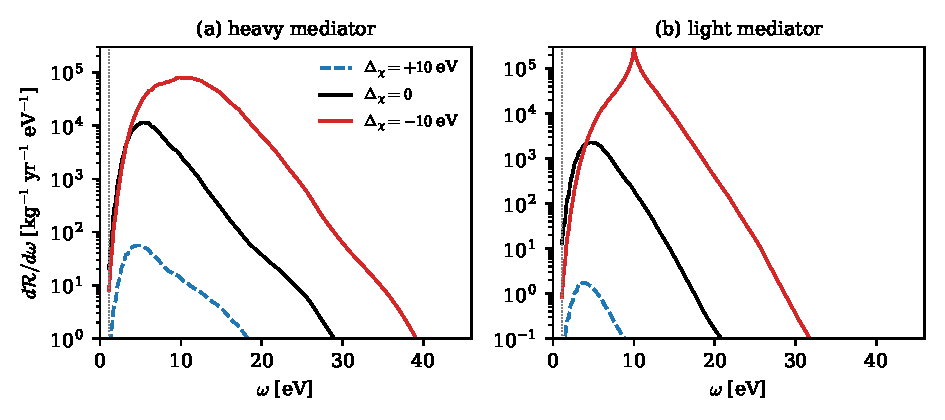
\includegraphics[width=\linewidth]{figures/ch10/fig10_8.pdf}
  \caption{Electron-recoil spectrum of silicon for inelastic dark matter of mass $\mchi = \SI{10}{MeV}$ with splittings $\Delta_\chi = \SI{+10}{eV}$ (endothermic, dashed), 0 (elastic) and \SI{-10}{eV} (exothermic), from \cref{eq:10.9-inel}. Inputs: the random-phase loss function with local fields of the tables of \cref{sec:10.2}, the standard halo of \cref{sec:1.2}, $\rho_\chi = \SI{0.3}{GeV.cm^{-3}}$ and $\sigmae = \SI{e-37}{cm^2}$. Dotted: \SI{1.11}{eV}, the step-model gap that accompanies the tables, below the low-temperature gap of \SI{1.17}{eV} to which their scissor shifts the bands. Below $|\vect{q}| = \SI{493}{eV}$, the first tabulated momentum, the loss function is held at its value there. (a) Heavy mediator, $\FDM = 1$. (b) Light mediator, $\FDM = (q_0/q)^2$; the exothermic spectrum peaks at $\omega = |\Delta_\chi|$, where the momentum transfer goes to zero.}
  \label{fig:10-inelastic}
\end{figure}

An exothermic particle is not limited by the kinetic energy of the halo, and its spectrum is set by the splitting. To see how, complete the square in $\omega_{\vect{q}}$ with $\Delta_\chi < 0$,
\begin{equation*}
  \omega_{\vect{q}} = |\Delta_\chi| + \vect{q}\cdot\vect{v} - \frac{q^2}{2\mchi} = |\Delta_\chi| + \tfrac12\mchi v^2 - \frac{|\vect{q} - \mchi\vect{v}|^2}{2\mchi} .
\end{equation*}
At fixed $\omega < |\Delta_\chi|$ the delta function of \cref{eq:8.2-spectrum} puts $\vect{q}$ on a sphere of radius $k_*$ centered at $\mchi\vect{v}$, with $k_*^2 = q_\Delta^2 + \mchi^2v^2$ and
\begin{equation*}
  q_\Delta = \sqrt{2\mchi\bigl(|\Delta_\chi| - \omega\bigr)} , \qquad v_\Delta = q_\Delta/\mchi .
\end{equation*}
For any function $G$ of $|\vect{q}|$, $\int\dd^3q\,\delta(\omega - \omega_{\vect{q}})\,G = \mchi k_*\int\dd^2\hat{\vect{n}}\,G(|\mchi\vect{v} + k_*\hat{\vect{n}}|)$. On the sphere $q^2 = k_*^2 + \mchi^2v^2 + 2k_*\mchi\vect{v}\cdot\hat{\vect{n}}$, and the term linear in $\vect{v}$ averages to zero because the sphere is centered at $\mchi\vect{v}$. The integral is therefore $4\pi\mchi q_\Delta G(q_\Delta)[1 + O(v^2/v_\Delta^2)]$, exactly $4\pi\mchi k_*G$ for constant $G$. The rate per particle no longer depends on its velocity, and the average over the halo is trivial. With $G = |\tilde V|^2\bar S$, $\bar S = (2q^2/e^2)\bar L$ and $\rho_\chi/\mchi\rho_T$ per unit mass,
\begin{keyresult}[Exothermic shell]
\begin{equation}
  \frac{\dd\mathcal{R}}{\dd\omega} = \frac{\rho_\chi\,\sigmae\,q_\Delta^3\,\FDM(q_\Delta)^2\,\bar L(q_\Delta,\omega)}{4\pi^2\alpha\,\rho_T\,\mu_{\chi e}^2}\,\Bigl[1 + O\bigl(v^2/v_\Delta^2\bigr)\Bigr] , \qquad \omega < |\Delta_\chi| ,
  \label{eq:10.9-shell}
\end{equation}
independent of the velocity distribution as long as $v_\Delta$ exceeds the speeds of the halo. The spectrum samples the response along the parabola $\omega = |\Delta_\chi| - q^2/2\mchi$.
\end{keyresult}
\noindent For constant $\bar L$ and a heavy mediator the correction is about $2.5\langle v^2\rangle/v_\Delta^2$, with $\langle v^2\rangle^{1/2} = 1.3\times10^{-3}$ in the laboratory frame: at $\mchi = \SI{0.1}{MeV}$ and $\omega = \SI{3}{eV}$, \cref{eq:10.9-inel} exceeds \cref{eq:10.9-shell} by \SI{2.9}{\percent}. Since $v_\Delta^2 = 2(|\Delta_\chi| - \omega)/\mchi$, the shell form needs $\mchi$ well below $2|\Delta_\chi|/v_{\mathrm{max}}^2$, which is \SI{2.9}{MeV} for $|\Delta_\chi| = \SI{10}{eV}$; at \SI{10}{MeV} the halo still matters, and \cref{fig:10-inelastic} uses \cref{eq:10.9-inel}.

The parabola explains where exothermic spectra peak. On a free electron at rest the response is a line, $S \propto \delta(\omega - q^2/2m_e)$, and it crosses the parabola once, at
\begin{equation*}
  \omega_{\mathrm{line}} = \frac{\mu_{\chi e}}{m_e}\,|\Delta_\chi| , \qquad q_{\mathrm{line}} = \sqrt{2\mu_{\chi e}|\Delta_\chi|} ,
\end{equation*}
the energy shared between the two recoiling particles. A heavy dark-matter particle hands the whole splitting to the electron, and a light one keeps part of it. In a crystal the electron line exists only where the free-electron picture holds, $q_{\mathrm{line}} \gg q_0$, that is $\omega_{\mathrm{line}} \gg q_0^2/2m_e = \SI{13.6}{eV}$. For smaller splittings the parabola crosses the region in which the response is that of bound electrons, and the peak sits where $q_\Delta^3\bar L$ is largest. The factor $q_\Delta^3$ falls toward $\omega = |\Delta_\chi|$, while $\bar L$ rises from the gap toward the plasma frequency, and the product peaks in between.

A light mediator turns the end of the spectrum into a line. As $\omega \to |\Delta_\chi|$, $q_\Delta \to 0$ and $\bar S \to (q^2/2\pi\alpha)L(0,\omega)$, the optical limit, so that with $\FDM^2 = q_0^4/q^4$
\begin{equation}
  \frac{\dd\mathcal{R}}{\dd\omega} \to \frac{\rho_\chi\,\sigmae\,q_0^4\,L(0,\omega)}{4\pi^2\alpha\,\rho_T\,\mu_{\chi e}^2\,q_\Delta} \propto \bigl(|\Delta_\chi| - \omega\bigr)^{-1/2} .
  \label{eq:10.9-edge}
\end{equation}
The divergence is integrable. Within $\tfrac12\mchi v^2$ of the end point, where $v_\Delta$ falls below the halo speeds, the exact kernel softens it to a logarithm, since there the momentum transfer can go to zero for every speed of the halo. Its strength is the optical loss function at $\omega = |\Delta_\chi|$: near the end point the exothermic particle acts like a boson of mass $|\Delta_\chi|$ absorbed at $\vect{q} \simeq 0$ (\cref{sec:8.2-exothermic}), and like the dark photon of \cref{sec:10.7} it reads $L$ rather than $\varepsilon_2$.

\begin{workedexample}{Exothermic lines in silicon}\label{we:10-exo}
Take $\Delta_\chi = \SI{-10}{eV}$ in silicon and the masses 0.1, 0.3, 1 and \SI{3}{MeV}. The free-electron lines would sit at $\omega_{\mathrm{line}} = 1.64$, 3.70, 6.62 and \SI{8.54}{eV}, at $q_{\mathrm{line}} = 1.29$, 1.94, 2.60 and \SI{2.96}{keV}. Every one of these momenta lies below $q_0 = \SI{3.73}{keV}$; even an infinitely heavy particle reaches only $q_{\mathrm{line}} = (2m_e|\Delta_\chi|)^{1/2} = \SI{3.20}{keV}$. A \SI{10}{eV} splitting therefore never meets free electrons in silicon.

The silicon spectrum from \cref{eq:10.9-inel}, with the random-phase loss function with local fields and a heavy mediator, peaks at 6.95, 6.19, 5.99 and \SI{7.29}{eV} for the four masses, with half-maximum edges between about 4 and \SI{8.5}{eV} (up to \SI{11.8}{eV} at \SI{3}{MeV}). At \SI{0.1}{MeV} the peak lies \SI{5.3}{eV} above the free-electron line, at \SI{1}{MeV} \SI{0.6}{eV} below it: the peak barely moves with the mass because it is set by the loss function, not by the recoil. The momentum transfer at the peak is $q_\Delta = 0.78$, 1.51, 2.83 and \SI{4.03}{keV}, from $0.21\,q_0$ to $1.08\,q_0$. Per kilogram-year at $\sigmae = \SI{e-37}{cm^2}$ the totals are $2.1\times10^5$, $3.1\times10^5$, $8.7\times10^5$ and $1.5\times10^6$. The shell form \cref{eq:10.9-shell} reproduces them to 0.91, 0.81, 0.63 and 0.73. The largest speeds of the halo reach $v_\Delta$ at the peak for $\mchi \gtrsim \SI{1}{MeV}$, with $v_{\mathrm{max}}/v_\Delta = 0.34$, 0.53, 0.94 and 1.97. At the lightest mass the residual comes from the tables: binned in \SI{100}{eV} steps of $|\vect{q}|$, the loss function varies by about \SI{15}{\percent} from bin to bin at these momenta, and the shell form samples a single $q$.

With a light mediator every mass gives a line at $\omega = \SI{10.0}{eV}$, an integrable cusp whose width is set by the energy resolution of the detector rather than by the halo. The last \SI{0.5}{eV} below $|\Delta_\chi|$ holds 40, 42, 47 and \SI{60}{\percent} of the rate, and the \SI{0.1}{eV} around $|\Delta_\chi|$ holds 15, 12, 8 and \SI{6.5}{\percent}. Its height follows from \cref{eq:10.9-edge} with $L(0,\SI{10}{eV})$, which is 0.247 measured (\cref{we:10-darkphoton}) and 0.218 in the first bin of the tables. The two mediators therefore leave different signatures for the same splitting: a broad bump near \SI{6}{eV} whose position hardly depends on the mass, or a line at the splitting itself. Neither sits at $\mu_{\chi e}|\Delta_\chi|/m_e$.
\end{workedexample}

Nothing new is needed from the material: \cref{eq:10.9-inel} uses the same loss functions as the elastic rate, now on a grid of $\omega$ that extends to $|\Delta_\chi| + \tfrac12\mchi v_{\mathrm{max}}^2$, and the light-mediator line needs the optical limit, which measurements give. Above \SI{99}{eV} the $2p$ shell of silicon opens (\cref{sec:10.6}), and the valence tables no longer suffice.

\subsection{Boosted dark matter}\label{sec:10.9-boosted}

A light halo particle can be accelerated after it leaves the halo's equilibrium. Cosmic-ray electrons and protons of MeV to GeV energies cross the dark-matter halo of the Galaxy, and a small fraction of them scatter on dark-matter particles along the way, which then carry kinetic energies comparable to their mass. The resulting flux at the Earth is the line-of-sight integral of the dark-matter density times the cosmic-ray flux and the scattering cross-section. For electrons, Liang and collaborators write it as $\dd\Phi_\chi/\dd T_\chi = D_{\mathrm{eff}}(\rho_\chi/\mchi)\int\dd T_e\,(\dd\sigma_{\chi e}/\dd T_\chi)(\dd\Phi_e/\dd T_e)$, with $T_\chi$ and $T_e$ the kinetic energies and $D_{\mathrm{eff}} = \SI{8.02}{kpc}$ an effective distance for a halo profile integrated to \SI{10}{kpc}~\cite[Eq.~(1)]{liang2025plasmon}. The flux is small, since only one halo particle in many meets a cosmic ray, but it reaches speeds close to that of light and with them energies far above $\tfrac12\mchi v_{\mathrm{max}}^2$.

The Sun accelerates a second component. Halo particles that fall into it scatter on the electrons of the solar core, at $1.57\times10^7$\,K at the center~\cite[Table~5]{bahcall2001solar}, whose thermal speed $(3T/m_e)^{1/2}$ is about 0.09. Some leave with speeds of that order, far above the escape speed of the Galaxy but well below that of light. The DAMIC-M collaboration, Dark Matter in CCDs (DAMIC) at Modane, has searched for this solar-reflected component~\cite{aggarwal2026constraints}. In both cases the halo average of \cref{eq:8.2-spectrum} is replaced by an average over the flux. For a flux that is isotropic in the laboratory, the number density per unit speed is $(\dd\Phi_\chi/\dd v)/v$, and the non-relativistic rate keeps its form with
\begin{equation*}
  \frac{\rho_\chi}{\mchi}\,\eta(\vmin) \;\to\; \int_{\vmin}\dd v\;\frac{1}{v^2}\,\frac{\dd\Phi_\chi}{\dd v} ,
\end{equation*}
the replacement of Ref.~\cite[Eqs.~(9)--(11)]{aggarwal2026constraints}. The real fluxes are anisotropic, the solar one pointing away from the Sun, and the angular average of the response that makes $\eta$ sufficient is then an assumption. For speeds near that of light the non-relativistic rows themselves must be checked.

The non-relativistic potential of \cref{sec:8.1} assumed that the energy deposited is small against the momentum transfer, so that the mediator acts instantaneously. For a relativistic particle $\omega$ can approach $q$, and the mediator must be kept whole. Take a vector mediator of mass $m_V$ coupled with strengths $y_\chi$ and $y_e$ to the dark-matter current $J^\mu_\chi = \bar u(p')\gamma^\mu u(p)$ and to the electron current $J^\mu_e = (n_e, \vect{j}_e)$. We write $\mathcal{Q} = |\vect{q}|$ for the momentum transfer, to keep it apart from the four-momentum, and $E_\chi = (p^2 + \mchi^2)^{1/2}$ for the energy, so that $\omega = E_\chi(\vect{p}) - E_\chi(\vect{p} - \vect{q})$ by \cref{eq:8.1-omega}. The amplitude is $y_\chi y_e(J^0_\chi n_e - \vect{J}_\chi\cdot\vect{j}_e)/(\mathcal{Q}^2 - \omega^2 + m_V^2)$. Both currents are conserved. For the target, \cref{eq:4.3-continuity} gives $\hat{\vect{q}}\cdot\vect{j}_e \to (\omega/\mathcal{Q})n_e$ between eigenstates; for the dark matter, the Dirac equation gives $\hat{\vect{q}}\cdot\vect{J}_\chi = (\omega/\mathcal{Q})J^0_\chi$. Splitting each spatial current into its part along $\hat{\vect{q}}$ and its transverse part, $\vect{J}_\chi\cdot\vect{j}_e = (\omega^2/\mathcal{Q}^2)J^0_\chi n_e + \vect{J}_{\chi\mathrm{T}}\cdot\vect{j}_{e\mathrm{T}}$, and the amplitude becomes
\begin{equation}
  y_\chi y_e\,\frac{J^0_\chi\,n_e\,(1 - \omega^2/\mathcal{Q}^2) - \vect{J}_{\chi\mathrm{T}}\cdot\vect{j}_{e\mathrm{T}}}{\mathcal{Q}^2 - \omega^2 + m_V^2} .
  \label{eq:10.9-amp}
\end{equation}
For a massless mediator the density term is $J^0_\chi n_e/\mathcal{Q}^2$, the instantaneous Coulomb interaction, and only the transverse term propagates at the speed of light. Retardation enters the density row of a massive mediator as the factor $(1 - \omega^2/\mathcal{Q}^2)$, and it comes from keeping the longitudinal current, which continuity ties to the density.

The density row needs the spin average of $|J^0_\chi|^2$. Write $\gamma\cdot p = \gamma^\mu p_\mu$ for the four-momentum $p = (E_\chi, \vect{p})$. The spinors of \cref{eq:C.15-spinor} obey $\sum_su(p,s)\bar u(p,s) = \gamma\cdot p + \mchi$, and the traces needed are $\Tr(\gamma^\mu\gamma^\nu) = 4g^{\mu\nu}$, $\Tr(\gamma^\mu\gamma^\nu\gamma^\rho\gamma^\sigma) = 4(g^{\mu\nu}g^{\rho\sigma} - g^{\mu\rho}g^{\nu\sigma} + g^{\mu\sigma}g^{\nu\rho})$, and zero for an odd number of matrices. Then
\begin{equation*}
  \begin{aligned}
  \frac12\sum_{s,s'}\bigl|\bar u(p',s')\gamma^0u(p,s)\bigr|^2 &= \frac12\Tr\bigl[(\gamma\cdot p' + \mchi)\gamma^0(\gamma\cdot p + \mchi)\gamma^0\bigr] \\
  &= 2\bigl(E_\chi E'_\chi + \vect{p}\cdot\vect{p}' + \mchi^2\bigr) = (2E_\chi - \omega)^2 - \mathcal{Q}^2 ,
  \end{aligned}
\end{equation*}
where the four-matrix trace gives $4(2E'_\chi E_\chi - p'\cdot p)$ with $p'\cdot p = E'_\chi E_\chi - \vect{p}'\cdot\vect{p}$, and the last step uses $E'_\chi = E_\chi - \omega$ and $2\vect{p}\cdot\vect{p}' = p^2 + p'^2 - \mathcal{Q}^2$. Dividing by the normalization $2E_\chi\cdot2E'_\chi$ of the two dark-matter states, squaring \cref{eq:10.9-amp} and writing the couplings through $\sigmae$ as in \cref{eq:1.4-Vsq},
\begin{keyresult}[Relativistic density row]
\begin{equation}
  \mathfrak{D}_{nn} = \frac{\pi\sigmae}{\mu_{\chi e}^2}\;\frac{(2E_\chi - \omega)^2 - \mathcal{Q}^2}{4E_\chi(E_\chi - \omega)}\;\Bigl(1 - \frac{\omega^2}{\mathcal{Q}^2}\Bigr)^2\left[\frac{q_0^2 + m_V^2}{\mathcal{Q}^2 - \omega^2 + m_V^2}\right]^2 ,
  \label{eq:10.9-Drel}
\end{equation}
which tends to $\pi\sigmae\FDM^2/\mu_{\chi e}^2$ as $v \to 0$. The rate per particle is \cref{eq:8.2-rate} with $S_{nn} = (2\mathcal{Q}^2/e^2)\bar L$, and per unit target mass $\dd\mathcal{R}/\dd\omega = \rho_T^{-1}\int\dd v\,v^{-1}(\dd\Phi_\chi/\dd v)\,\dd\varGamma/\dd\omega$ for an isotropic flux.
\end{keyresult}
\noindent This constructs the relativistic tensor that \cref{sec:8.2-absorption} left open, for the density row. The transverse row enters through $\vect{J}_{\chi\mathrm{T}}$, whose square for a particle much heavier than the energy deposited is $4E_\chi^2v_{\mathrm{T}}^2$, with $v_{\mathrm{T}}^2 = v^2 - (\vect{v}\cdot\hat{\vect{q}})^2 = v^2 - \omega^2/\mathcal{Q}^2$. For a massless mediator the medium answers a transverse current through its transverse dielectric function $\varepsilon^{\mathrm{T}}$ of \cref{sec:4.4}, and the propagator $1/\mathcal{Q}^2$ of the density row becomes $1/(\mathcal{Q}^2 - \omega^2\varepsilon^{\mathrm{T}})$ in the transverse row. After averaging over the directions of $\vect{q}$ the density and the transverse current are uncorrelated, and the two rows add. The loss function of the density row is replaced by
\begin{equation}
  \bar L(\mathcal{Q},\omega) \;\to\; \bar L(\mathcal{Q},\omega) + \Bigl(v^2 - \frac{\omega^2}{\mathcal{Q}^2}\Bigr)\Imag\left[\frac{-\mathcal{Q}^2}{\omega^2\varepsilon^{\mathrm{T}}(\mathcal{Q},\omega) - \mathcal{Q}^2}\right] ,
  \label{eq:10.9-fermi}
\end{equation}
the form of Fermi's energy-loss formula for a fast charge~\cite{fermi1940ionization}, which a calculation of the transverse response of silicon writes for dark matter~\cite[Eq.~(2)]{liang2026dielectric}.

We can bound the retardation factor. For any particle whose energy is a convex function of its momentum, $E_\chi(p) - E_\chi(p') \le (\dd E_\chi/\dd p)(p - p')$, and $p - p' \le \mathcal{Q}$ by the triangle inequality, so
\begin{equation}
  \omega \le v\,\mathcal{Q} , \qquad \Bigl(1 - v_{\chi,\mathrm{max}}^2\Bigr)^2 \le \Bigl(1 - \frac{\omega^2}{\mathcal{Q}^2}\Bigr)^2 \le 1 ,
  \label{eq:10.9-bound}
\end{equation}
with $v_{\chi,\mathrm{max}}$ the largest speed in the flux. A rate computed without the factor is therefore too large by at most $(1 - v_{\chi,\mathrm{max}}^2)^{-2}$. For speeds up to 0.1 this is \SI{2}{\percent}, and up to 0.2 it is \SI{9}{\percent}. For the solar-reflected flux, with typical speeds of 0.1, the non-relativistic rate with $\eta$ replaced by the flux integral therefore stands at the level of a few percent. For cosmic-ray-boosted dark matter, with $v \to 1$, the bound says nothing, and the answer depends on where in $(\mathcal{Q},\omega)$ the rate collects.

For a heavy mediator the rate of silicon collects at $\mathcal{Q}$ of keV, where $\omega/\mathcal{Q}$ is tiny: the factor $(1 - \omega^2/\mathcal{Q}^2)^2$ changes the rate by $10^{-4}$ and the transverse row by at most $10^{-4}$. For a massless mediator the density row without the factor, $q_0^4/(\mathcal{Q}^2 - \omega^2)^2$, grows without limit as $\mathcal{Q} \to \omega$, where the exact longitudinal interaction is the Coulomb $q_0^4/\mathcal{Q}^4$; this form, with the mediator form factor evaluated at the four-momentum transfer, is the one of Ref.~\cite[Eqs.~(4)--(6)]{liang2025plasmon}. For a particle of speed $v$ the exact density row of silicon is then 0.997 of the row without the factor at $v = 0.1$, 0.94 at 0.5, 0.65 at 0.9 and 0.17 at 0.99 (\cref{fig:10-boost-limit}).

The transverse row of \cref{eq:10.9-fermi} contains the Cherenkov term of Fermi's formula, standard for fast charged particles in matter and in the photo-absorption-ionization model of energy loss in silicon~\cite{fermi1940ionization,allison1980relativistic}. Between the gap and the direct gap silicon is nearly transparent, with $\varepsilon_1 = 12.5$ at the gap rising to 44.9 at \SI{3.3}{eV} in the measured data at \SI{300}{K}. A particle faster than the light of the medium, $v > \varepsilon_1^{-1/2}$, which is 0.28 at \SI{1.2}{eV} and 0.15 at \SI{3.3}{eV}, emits Cherenkov radiation. The condition $\omega^2\varepsilon_1 = \mathcal{Q}^2$ is then met inside the kinematic range $\mathcal{Q} \ge \omega/v$, and the transverse term has a pole there, broadened only by the small $\varepsilon_2$. We take the measured $\varepsilon$ in place of $\varepsilon^{\mathrm{T}}$, valid at these small $\mathcal{Q}$, and a massless mediator. Below \SI{2}{eV} the transverse row then exceeds the density row, which is suppressed there by $1/|\varepsilon|^2$, by a factor of 49 at $v = 0.3$ and 530 at $v = 0.5$. Integrated over the spectrum above the gap, the transverse share is $2.7\times10^{-5}$ at $v = 0.1$, \SI{1}{\percent} at 0.5 and \SI{5.5}{\percent} at 0.99; in the plasmon window of 10 to \SI{20}{eV} it is $7\times10^{-4}$ at 0.5 and $7\times10^{-3}$ at 0.99. The Cherenkov photons are real photons, and they make electron--hole pairs only where the crystal absorbs them, within $1/(2\omega\Imag n_r)$, which is \SI{0.4}{mm} at \SI{1.2}{eV} and \SI{12}{\micro m} at \SI{1.5}{eV} in the warm data and longer in a cold crystal (\cref{sec:10.7-edge}). Whether they count is a question of the size and temperature of the detector.

\begin{figure}[tbp]
  \centering
  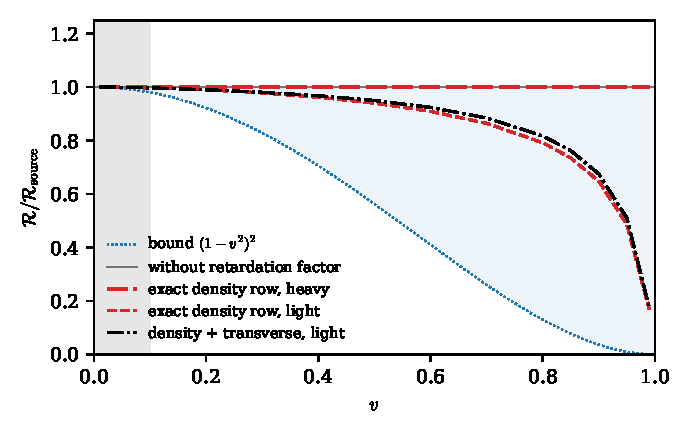
\includegraphics[width=0.82\linewidth]{figures/ch10/limit10_9b.pdf}
  \caption{Electron-recoil rate of silicon for dark matter of speed $v$, much heavier than the energy deposited, divided by the rate of the density row without the factor $(1 - \omega^2/\mathcal{Q}^2)^2$, against $v$. Red, long dashes: the exact density row \cref{eq:10.9-Drel} with a heavy mediator, which coincides with it to $10^{-4}$; red, short dashes: the same with a massless mediator; dash-dotted: the massless mediator with the transverse row of \cref{eq:10.9-fermi} added. Blue band: the range $[(1 - v^2)^2, 1]$ allowed by \cref{eq:10.9-bound}. Gray: $v \le 0.1$, where the bound guarantees agreement to \SI{2}{\percent}. Rates are integrated over $\omega$ from \SI{1.11}{eV}, the step-model gap that accompanies the tables, to \SI{89}{eV} and over $\mathcal{Q}$ from $\omega/v$ to \SI{22.5}{keV}. Loss function: random-phase with local fields, from the tables of \cref{sec:10.2}, held at its value at \SI{493}{eV} below that momentum. Transverse function: the measured $\varepsilon(\omega)$ of silicon at \SI{300}{K}~\cite{franta2017temperature}, with its Cherenkov pole integrated exactly; the transverse row counts the Cherenkov photons emitted above the gap as deposited energy, wherever they are absorbed.}
  \label{fig:10-boost-limit}
\end{figure}

\subsection{Fermionic absorption on electrons}\label{sec:10.9-fermionic}

A fermion $\chi$ of \SI{100}{keV} that is absorbed on an electron and leaves as a massless $\tilde\nu$ deposits $\omega = \mchi - q$ (\cref{eq:8.1-omega-ferm}). On a free electron at rest this is the recoil $q^2/2m_e$, so $q \simeq \mchi$ and $\omega \simeq \mchi^2/2m_e = \SI{9.8}{keV}$, a deposit that no halo particle of that mass could give by scattering. The momentum transfer is set by the rest energy and not by the speed of the dark matter, so that the rate is a single line through the response, independent of the halo. \Cref{sec:8.2-absorption} showed that the master formula holds with a sum over the momenta of $\tilde\nu$ and left the dark-matter tensor to be built here.

Take the operators $\Lambda_F^{-2}(\bar{\tilde\nu}P_L\chi)(\bar\psi\psi)$ and $\Lambda_F^{-2}(\bar{\tilde\nu}\gamma_\mu P_R\chi)(\bar\psi\gamma^\mu\psi)$ of \cref{sec:8.1-absorption}, with the chirality projectors $P_{L,R} = (1 \mp \gamma^5)/2$. Let $p = (\mchi, \vect{0})$ be the four-momentum of $\chi$ at rest and $k = (q, -\vect{q})$ that of $\tilde\nu$, so that $k\cdot p = \mchi q$. On the target side the scalar bilinear is the density row $n_e$ and the vector bilinear the current $J^\mu_e = (n_e, \vect{j}_e)$, up to terms of order $q/m_e$ (\cref{eq:C.15-bilinears}). On the dark-matter side, averaged over the spin of $\chi$ and summed over that of $\tilde\nu$, and with the trace identities of \cref{sec:10.9-boosted} together with $\Tr(\gamma^\mu\gamma^\nu\gamma^5) = 0$ and $P_L(\gamma\cdot p + \mchi)P_R = (\gamma\cdot p)P_R$,
\begin{gather*}
  \frac12\Tr\bigl[(\gamma\cdot k)P_L(\gamma\cdot p + \mchi)P_R\bigr] = k\cdot p = \mchi q , \\
  \frac12\Tr\bigl[(\gamma\cdot k)\gamma^\mu(\gamma\cdot p)\gamma^\nu P_L\bigr] = k^\mu p^\nu + k^\nu p^\mu - g^{\mu\nu}k\cdot p + \ii\epsilon^{\mu\nu\alpha\beta}k_\alpha p_\beta ,
\end{gather*}
up to the sign convention of the antisymmetric term. That term pairs with an antisymmetric current response, which a target with inversion symmetry and without magnetic order does not have, and we drop it. The relativistic normalization of the two dark-sector states divides by $2\mchi\cdot2q$. For the scalar operator the tensor is the number $\mathfrak{D}_{nn} = 1/4\Lambda_F^4$. For the vector operator, $\mathfrak{D}^{00} = 1/4\Lambda_F^4$, $\mathfrak{D}^{0i} = -q^i/(4q\Lambda_F^4)$ and $\mathfrak{D}^{ij} = \delta^{ij}/4\Lambda_F^4$, contracted with the responses of $J_\mu = (n_e, -\vect{j}_e)$. Continuity, $\hat{\vect{q}}\cdot\vect{j}_e \to (\omega/q)n_e$, turns the longitudinal current into the density, and the density, cross and longitudinal terms add to $(1 + \omega/q)^2S_{nn} = (\mchi/q)^2S_{nn}$. The transverse current, two components, keeps the weight one. With $\dd^3q/(2\pi)^3 = q^2\dd\omega/2\pi^2$ along the line $q = \mchi - \omega$, and with $\sigma_F = \mchi^2/4\pi\Lambda_F^4$,
\begin{keyresult}[Fermionic absorption on electrons]
\begin{equation}
  \begin{gathered}
  \frac{\dd\varGamma_S}{\dd\omega} = \frac{\sigma_F}{2\pi}\,\frac{q^2}{\mchi^2}\,\bar S_{nn}(q,\omega) , \\
  \frac{\dd\varGamma_V}{\dd\omega} = \frac{\sigma_F}{2\pi}\Bigl[\bar S_{nn}(q,\omega) + \frac{q^2}{\mchi^2}\,\Tr\bar S_{\vect{j}_{\mathrm{T}}\vect{j}_{\mathrm{T}}}(q,\omega)\Bigr] , \qquad q = \mchi - \omega ,
  \end{gathered}
  \label{eq:10.9-ferm}
\end{equation}
for the scalar and vector operators, at $v \to 0$ and for a massless $\tilde\nu$; the event rate per unit mass is $(\rho_\chi/\mchi\rho_T)\varGamma$, independent of the velocity distribution.
\end{keyresult}
\noindent For free electrons at rest, $\bar S_{nn} = 2\pi\nd_e\delta(\omega - q^2/2m_e)$ and the transverse current vanishes, and both rates are $\nd_e\sigma_F$ up to corrections of relative order $\mchi/m_e$, from the recoil of the electron~\cite[Eqs.~(1), (2) and (10)]{dror2021absorption}.

For an atomic shell the density response is the ionization form factor of \cref{eq:2.2-fion}: with the binding energy $E_B$ and the ejected energy $E_{\mathrm{ej}} = \omega - E_B$, the response per atom is $\pi|f_{\mathrm{ion}}(p_{\mathrm{ej}},q)|^2/2E_{\mathrm{ej}}$, both spins counted in $|f_{\mathrm{ion}}|^2$ as in Ref.~\cite[Eqs.~(A.18)--(A.21)]{essig2016direct}. The scalar rate of \cref{eq:10.9-ferm} then becomes $\dd\langle\sigma v\rangle_S/\dd E_{\mathrm{ej}} = \sigma_Fq^2|f_{\mathrm{ion}}|^2/(4E_{\mathrm{ej}}\mchi^2)$.

A light mediator changes the rate in a way that the dark-matter speed does not control. For the scalar operator mediated by a scalar of mass $m_{\mathrm{med}}$ with Yukawa couplings $y_{ee}$ and $y_{\chi\tilde\nu}$, $\Lambda_F^{-2}$ becomes $y_{ee}y_{\chi\tilde\nu}/(m_{\mathrm{med}}^2 - t)$, with $t$ the squared four-momentum transfer. On the $\tilde\nu$ leg, $t = (p - k)^2 = \omega^2 - q^2 = 2\mchi\omega - \mchi^2$, fixed by the rest energy, unlike the $-q^2$ of scattering. The rate is then the contact rate times $[m_{\mathrm{med}}^2/(m_{\mathrm{med}}^2 + \mchi^2 - 2\mchi\omega)]^2 = 1 - 2(\mchi^2 - 2\mchi\omega)/m_{\mathrm{med}}^2 + \dots$, the correction of relative order $(\mchi/m_{\mathrm{med}})^2$ that Cox, Dolan and Wood attach to the contact limit~\cite[Eqs.~(1), (2), (14) and (15)]{cox2024absorption}. It also tilts the spectrum, raising the high-$\omega$ end.

The two halves of this section meet when $\tilde\nu$ is massive. With $m_{\tilde\nu} = \mchi + \Delta_\chi$ and $|\Delta_\chi| \ll \mchi$, the outgoing fermion is slow, and \cref{eq:8.1-omega-inel} gives $\omega$ exactly as for inelastic scattering, with the recoil term computed with $\mchi$ instead of $m_{\tilde\nu}$ and the tensor multiplied by $\mchi/m_{\tilde\nu}$, both corrections of relative order $\Delta_\chi/\mchi$ (\cref{app:D.24}). Absorption into a nearly degenerate fermion is exothermic or endothermic scattering, and \cref{eq:10.9-inel} applies.

In practice the responses on the line $\omega = \mchi - q$ reach far above the valence scale. For $\mchi$ from the gap to \SI{1}{MeV} the momentum transfer runs into the cores of the atoms. The density row and the transverse current row are then needed from all-electron states, with Dirac--Hartree--Fock orbitals where $q \gtrsim m_e/3$.

\subsection{In-medium decay of an excited state}\label{sec:10.9-decay}

An excited state $\chi_2$ that survives from the early universe, or that a scattering in the Earth produces, can decay to $\chi_1$ inside the detector without touching anything, emitting a photon of energy $|\Delta_\chi|$. A transition magnetic moment $\mu_{\mathrm{M}}$ between the two states, $H = -\mu_{\mathrm{M}}\boldsymbol{\sigma}\cdot\vect{B}$ with $\boldsymbol{\sigma}$ the Pauli matrices between the spin states of $\chi_2$ and $\chi_1$, gives the vacuum rate
\begin{equation}
  \varGamma_{\mathrm{vac}} = \frac{\mu_{\mathrm{M}}^2|\Delta_\chi|^3}{\pi} ,
  \label{eq:10.9-vac}
\end{equation}
for $|\Delta_\chi| \ll \mchi$. This is the electric-dipole rate $\omega^3|\vect{d}|^2/3\pi$ of Heaviside--Lorentz units, with $|\vect{d}|^2$ replaced by the spin sum $\mu_{\mathrm{M}}^2\sum_f|\langle f|\boldsymbol{\sigma}|i\rangle|^2 = 3\mu_{\mathrm{M}}^2$. Baryakhtar and collaborators estimate the lifetime for a dipole operator $\bar\chi_2\sigma^{\mu\nu}\chi_1F_{\mu\nu}$ with coefficient $1/\Lambda_d$ as $\tau^{-1} \sim \pi|\Delta_\chi|^3/\Lambda_d^2$~\cite[Eqs.~(2.1) and (2.2)]{baryakhtar2020electromagnetic}. In the non-relativistic limit $\sigma^{\mu\nu}F_{\mu\nu} \to -2\boldsymbol{\sigma}\cdot\vect{B}$, so that $\mu_{\mathrm{M}} \simeq 2/\Lambda_d$, and \cref{eq:10.9-vac} gives $4|\Delta_\chi|^3/\pi\Lambda_d^2$, the same scaling. No operator of the target appears in the amplitude, and the master formula does not apply as it stands. The medium enters through the photon.

The decay rate follows from the golden rule with the magnetic field of the medium as the final state. At $T = 0$ the spectral density of the field is twice the imaginary part of its propagator, and in a medium the transverse propagator is $1/(\mathcal{Q}^2 - \omega^2\varepsilon^{\mathrm{T}})$, with $\vect{B} = \ii\vect{q}\times\vect{A}$. The spin average gives $\frac12\Tr(\sigma^i\sigma^j) = \delta^{ij}$, the transverse projection of $\vect{q}\times\vect{A}$ gives $2\mathcal{Q}^2$, and with $\omega = |\Delta_\chi|$, neglecting the recoil of $\chi_1$,
\begin{equation}
  \varGamma = \frac{2\mu_{\mathrm{M}}^2}{\pi^2}\int_0^\infty\dd\mathcal{Q}\;\mathcal{Q}^4\,\Imag\frac{1}{\mathcal{Q}^2 - \omega^2\varepsilon^{\mathrm{T}}(\mathcal{Q},\omega)} .
  \label{eq:10.9-decay}
\end{equation}
In vacuum $\Imag[1/(\mathcal{Q}^2 - \omega^2 - \ii0)] = \pi\delta(\mathcal{Q}^2 - \omega^2)$, and \cref{eq:10.9-decay} returns \cref{eq:10.9-vac}. In a transparent medium, $\varepsilon_2 \to 0$, the delta function sits at $\mathcal{Q} = \omega n_r$ with the refractive index $n_r = \sqrt{\varepsilon}$, and the rate is $n_r^3\varGamma_{\mathrm{vac}}$. The same calculation with the electric field, $\vect{E} = \ii\omega\vect{A}$, gives $n_r\varGamma_{\mathrm{vac}}$ for an electric dipole, local-field factors aside. The difference has a simple reason: the density of photon states grows as $n_r^2$ times the group index $n_{\mathrm{grp}}$, the electric field per photon falls as $1/(n_rn_{\mathrm{grp}})$, and the magnetic field per photon is $n_r$ times the electric one.

Where the medium absorbs, \cref{eq:10.9-decay} changes character. At large $\mathcal{Q}$ the integrand tends to $\omega^2\varepsilon_2^{\mathrm{T}}$, and the integral grows with the momentum up to which $\varepsilon_2^{\mathrm{T}}(\mathcal{Q},\omega)$ stays finite. That large-momentum part is not a photon. It is energy handed directly to the electrons near the particle through a virtual photon, a scattering $\chi_2 + \text{target} \to \chi_1 + \text{excitation}$. Its rate is the master formula with $\Delta_\chi < 0$, the magnetic-dipole operators of \cref{sec:8.1} and the transverse current row: the exothermic process of \cref{sec:10.9-inelastic} with a different vertex. The decay thus splits at an interface. The radiative part, a photon of energy $|\Delta_\chi|$ that is absorbed later or escapes, lies outside the response picture and is listed among the processes outside the framework in \cref{sec:22.3}. The non-radiative part lies inside it and needs $\varepsilon^{\mathrm{T}}$, or the transverse current response, at finite $\mathcal{Q}$.

Silicon shows the three regimes. Below the gap it is transparent, with $n_r = 3.44$ at \SI{0.5}{eV} and 3.54 at \SI{1.1}{eV}, and an excited state with a splitting there decays $n_r^3 = 41$ to 44 times faster inside the crystal than in vacuum, into a photon that the crystal does not absorb. Between 3.2 and \SI{22.5}{eV}, where $\Imag n_r > 0.1\Real n_r$, the decay is non-radiative, and its rate is the master-formula rate. Above the plasma frequency $n_r$ approaches one, from below as $1 - \omega_p^2/2\omega^2$ for a free electron gas and with small excursions at the $2p$ edge, and the vacuum rate holds within \SI{10}{\percent} for every splitting above \SI{55}{eV}.

\begin{limitbox}[In-medium decay of an excited state][lim:10.9d]
Vacuum decay through a transition dipole: $\tau^{-1} \sim \pi|\Delta_\chi|^3/\Lambda_d^2$ for the operator $(1/\Lambda_d)\bar\chi_2\sigma^{\mu\nu}\chi_1F_{\mu\nu}$~\cite[Eqs.~(2.1) and (2.2)]{baryakhtar2020electromagnetic}, in the book's form $\varGamma_{\mathrm{vac}} = \mu_{\mathrm{M}}^2|\Delta_\chi|^3/\pi$ (\cref{eq:10.9-vac}) with $\mu_{\mathrm{M}} \simeq 2/\Lambda_d$.
\par\smallskip
{\centering
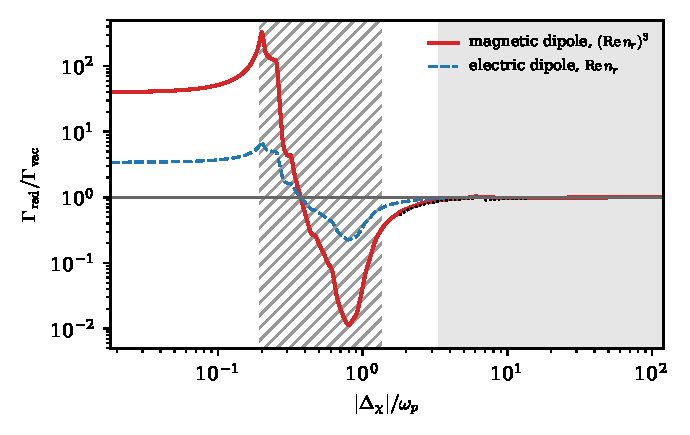
\includegraphics[width=0.82\linewidth]{figures/ch10/limit10_9d.pdf}
\captionof{figure}{Radiative decay rate of an excited state inside silicon over the vacuum rate, against the splitting $|\Delta_\chi|$ in units of the valence plasma frequency $\omega_p^{\mathrm{val}} = \SI{16.6}{eV}$. Red: magnetic dipole, $(\Real n_r)^3$; blue dashed: electric dipole, $\Real n_r$, local-field factors omitted. $n_r = \sqrt{\varepsilon}$ from the measured dielectric function of silicon at \SI{300}{K} below \SI{40}{eV}~\cite{franta2017temperature} and from atomic scattering factors above~\cite{henke1993xray}. Dotted: the free-electron-gas asymptote $n_r^3 \simeq 1 - 3\omega_p^2/2\omega^2$, with $\omega_p^{\mathrm{val}}$ below the $2p$ edge and the all-electron \SI{31.1}{eV} above. Hatched: $\Imag n_r > 0.1\Real n_r$, 3.2 to \SI{22.5}{eV}, where the radiative factor loses its meaning and the decay is a non-radiative transfer given by \cref{eq:10.9-decay} at finite $\mathcal{Q}$. Gray: splittings above \SI{55}{eV}, $3.3\,\omega_p^{\mathrm{val}}$, where $(\Real n_r)^3$ is within \SI{10}{\percent} of one.}\label{fig:10-decay-limit}
\par}
\smallskip
Below about $3\omega_p^{\mathrm{val}}$ the vacuum rate fails inside a solid: it is enhanced by $n_r^3 \approx 40$ in the transparent window of silicon below the gap and replaced by non-radiative transfer to the electrons where the crystal absorbs.
\end{limitbox}

\noindent No response of the target enters the vacuum rate; the medium acts only through $\varepsilon^{\mathrm{T}}$ at $\mathcal{Q} = \omega n_r$, and in a transparent medium the leading correction is the local field at the particle, which the macroscopic $\varepsilon$ does not contain.
